% IEEE standard conference template; to be used with:
%   spconf.sty  - LaTeX style file, and
%   IEEEbib.bst - IEEE bibliography style file.
% --------------------------------------------------------------------------

\documentclass[letterpaper]{article}
\usepackage{spconf,amsmath,amssymb,graphicx}

% Example definitions.
% --------------------
% nice symbols for real and complex numbers
\newcommand{\R}[0]{\mathbb{R}}
\newcommand{\C}[0]{\mathbb{C}}

% bold paragraph titles
\newcommand{\mypar}[1]{{\bf #1.}}

\newcommand{\fixme}[1]{{\bf FIXME}: {\it #1}}
\newcommand{\comment}[1]{}

% Title.
% ------
\title{Optimizing Domain Trasform for Edge-Aware Image Processing}
%
% Single address.
% ---------------
\name{Adrian Blumer, Pascal Sp\"orri, Julia Pe\v{c}erska\comment{\thanks{The author thanks Jelena Kovacevic. This paper
is a modified version of the template she used in her class.}}} 
\address{Department of Computer Science\\ ETH Z\"urich\\Z\"urich, Switzerland}

\begin{document}
%\ninept
%
\maketitle
%

\begin{abstract}
\fixme{Review and shorten}

Edge-aware filtering can be used as a basic building block for many image processing tasks. In this field of research the recent publication \textit{Domain Transform for Edge-Aware Image and Video Processing} ~\cite{GastalOliveira2011DomainTransform} introduces a new and promising algorithm. 

At the time of writing of this report, the only publicly avaiable implementation of this method is a Matlab version provided by the papers authors.

The goal of this project is to provide a performant C/C++ implementation of the aforementioned method, while documenting and discussing both our successfull and failed optimisation approaches.
Starting with a direct port of the Matlab code, we apply various optimisations to achieve an approximate $2$ times speedup with regard to our base version. Optimisation potential still exists as we are far from both memory and computation bounds, however neither of our further optimisation attempts get us closer to these bounds. 

\comment{
Describe in concise words what you do, why you do it (not necessarily
in this order), and the main result.  The abstract has to be
self-contained and readable for a person in the general area. You
should write the abstract last.
}
\end{abstract}



\section{Introduction}\label{sec:intro}
\fixme{Review}

Filtering operations are often a crucial step of image processing. In
particular, most useful filter options are edge-aware smoothing filters, 
whose output can be used as a building block for multiple other applications.
For example, such filters can be used to extract or remove features from an
image, to colorize the image in a intuitive fashion by colouring specific
items on an image, as well as perform other tasks such as noise removal and
image compression.

As in most cases with image (and in particular with video) processing, it is
highly required that the filters have a low computational cost and therefore
can produce fast results, especially when used for real-time transformation of
graphical data. It is also true that image recording technologies advance and 
therefore can create images of greater resolution, which means an increase in
the amount of computation needed for filtering. And lastly images are 2D data
and will have to be processed both horizontally and vertically, which makes
spatial locality troublecome.

There exist multiple algorithms that perform this type of filtering, however
most of these are computationally heavy and almost impossible to execute in
real-time. Moreover, some of those only naturally support grayscale images. \fixme{should we add references here?}
For this project we have picked one of the fastest known algorithms for the
task in question, which works on full RGB images.

The main idea of this fast approach is to use a domain transformation on the
image which allows to reduce the dimensionality of the data. An RGB image in
essence is a 2D manifold in 5D space, and an edge-preserving filter can be
defined in lower dimensions as long as the 5D distances among the pixels are
preserved. The transformation defines an isometry between curves on the 2D
manifold and the real line. It preserves the geodesic distance between points
on the curve wrapping the image into two 1D domains, one for horizontal 
distances and one for vertical. Then a 1D edge-preserving filter can be ran on
this transformed domain.

The work presented here aims at optimizing the implementation of on of the 
more sophisticated algorithm versions on the CPU. The only publicly available
implementation of it is in MATLAB, and is useless for fast prosessing of image
data. We have implemented the algorith in C/C++ and proceeded to use the
techniques described in the course to improve its performance.

\comment{Do not start the introduction with the abstract or a slightly modified
version. It follows a possible structure of the introduction. 
Note that the structure can be modified, but the
content should be the same. Introduction and abstract should fill at most the first page, better less.

\mypar{Motivation} The first task is to motivate what you do.  You can
start general and zoom in one the specific problem you consider.  In
the process you should have explained to the reader: what you are doing,
why you are doing, why it is important (order is usually reversed).

For example, if my result is the fastest DFT implementation ever, one
could roughly go as follows. First explain why the DFT is important
(used everywhere with a few examples) and why performance matters (large datasets,
realtime). Then explain that fast implementations are very hard and
expensive to get (memory hierarchy, vector, parallel). 

Now you state what you do in this paper. In our example: 
presenting a DFT implementation that is
faster for some sizes than all the other ones.

\mypar{Related work} Next, you have to give a brief overview of
related work. For a paper like this, anywhere between 2 and 8
references. Briefly explain what they do. In the end contrast to what
you do to make now precisely clear what your contribution is.
}

\section{Background: Whatever the Background is}\label{sec:background}
\fixme{Review.}

In this section we will present the necessary background information to follow our implementation of the \textit{Normalized convolution} domain transform filtering algorithm. For a more detailed explanation of the method and its theoretical background, please refer to the original ~\cite{GastalOliveira2011DomainTransform}.

The straight forward approach to image bluring is to compute a new value for each image pixel using the weighted average of its neighbourhood. To decide whether a pixel lies in this neighbourhood, we need some kind of distance measure. In the case of simple edge unaware bluring (such as applying a Gaussian filter), this distance measure is the spatial distance between image pixels. However to achieve edge-aware image filtering the radiometric distance between pixels (their difference in color) has to be taken into account as well.
In general this increases the dimensionality of the problem by adding a dimension for each color channel.

For a RGB color image this would lead to a 5-dimensional space (3 radiometric + 2 spatial dimensions). The domain transform method reduces this dimensionality as follows:
First, it treats the two spatial dimensions separately. What this means is that the image is separately filtered along its rows and columns. Secondly, it merges the three radiometric dimensions and the remaining one spatial dimension into the one-dimensional space of the domain transform. This transformation retains the necessary distance properties from the original space.

Looking at a single image row, the pixels can be enumerated from left to right as $ p_0 \dots p_n$. Each pixel $p_i$ is associated with a domain transform value $dt_i$ where it holds that $\forall k : dt_k \leq dt_{k+1}$. In other words, the series of domain transform values is monotonically increasing. The exact difference between two consecutive domain transform values depends on the pixels spatial and radiometric distance.



\mypar{Cost Analysis}
In asymptotic terms, the algorithm has a complexity of \BigO{n}, which makes it already very competitive with other approaches to edge-aware image filtering. For optimization purposes we are however interested in a more thorough cost analysis of the method. Therefore we have counted the number of different floating point operations executed by the algorithm:

\setlength\fboxsep{0pt}
\setlength\fboxrule{0.5pt}

\begin{figure}\vspace{-1mm}
  \includegraphics[trim=10mm 145mm 100mm 10mm, clip, width=0.48\textwidth]{figures/flowchart.pdf}
  \caption{Algorithm flowchart\label{flowchart}}
\end{figure}

\comment{
Give a short, self-contained summary of necessary
background information. For example, assume you present an
implementation of FFT algorithms. You could organize into DFT
definition, FFTs considered, and cost analysis. The goal of the
background section is to make the paper self-contained for an audience
as large as possible. As in every section
you start with a very brief overview of the section. Here it could be as follows: In this section 
we formally define the discrete Fourier transform, introduce the algorithms we use
and perform a cost analysis.

\mypar{Discrete Fourier Transform}
Precisely define the transform so I understand it even if I have never
seen it before.

\mypar{Fast Fourier Transforms}
Explain the algorithm you use.

\mypar{Cost Analysis}
First define you cost measure (what you count) and then compute the
cost. Ideally precisely, at least asymptotically. In the latter case you will need to instrument your code to count
the operations so you can create a performance plot.

Also state what is
known about the complexity (asymptotic usually) 
about your problem (including citations).

Don't talk about "the complexity of the algorithm.'' It's incorrect,
remember (Lecture 2)?
}

%\section{Your Proposed Method}\label{sec:method}
\section{Optimizing Domain Transform}

This section describes the baseline implementation of the algorithm and the optimisation steps we executed that made a significant impact on the performance of the code. Finally the section also describes and discusses further optimisation approaches that were tried out and discarded because they didn't lead to a performance improvement.

\subsection{Baseline version}

Our baseline implementation is a straightforward port to C++ of the Matlab code provided on the homepage\footnote{\url{http://www.inf.ufrgs.br/~eslgastal/DomainTransform/}} of the authors of the paper describing the algorithm~\cite{GastalOliveira2011DomainTransform}.
\begin{lstlisting}[caption=Matrix struct,label=code:matrix_struct]
struct Mat2
{
    uint width, height;
    float3* data; // size: width*height
};
\end{lstlisting}

In order to preserve the precision of calculations all images are store using a \lstinline{float3} struct, which uses $3\times 4 = 12$ bytes per pixel. Hence a $1$M pixel image is stored in $3\times 4\times 10^6$\ B $=12$\ MB.

The algorithm starts with some initialisation procedures. During initialisation two matrices - $dIdx$ and $dIdy$ - are precomputed, which contain the differentials of the neighbouring image pixels in both $x$ and $y$ directions. Afterwards a prefix sum is computed for both $dIdx$ and $dIdy^T$, creating matrices which in fact contain for each pixel a mapping into 1D coordinate space along each direction.

During the filtering step (see listing~\ref{code:filterstep}) we compute \texttt{comp\-ute\ Bound} and \texttt{boxFilter} twice. After each computation step we transpose the images.

\begin{lstlisting}[caption=Filterstep,label=code:filterstep]
for (i=0; i<iterations; i++)
    bounds = computeBound(img, dIdX, r);
    img = boxFilter(img, bounds);
    img = transpose(img);
    bounds = computeBound(img, dIdY, r);
    img = boxFilter(img, dIdY, bounds);
    img = transpose(img);
\end{lstlisting}

The \lstinline{computeBound} method computes the 1D upper and lower bound for the box filter of each pixel, which is dependent on the predefined filter radius. 

Before the actual application of the box filter, a prefix sum over the image pixels is computed. This cannot be done once for the whole algorithm and needs to be recomputed, as the pixel values change between iterations. Then the \lstinline{boxFilter} makes use of the previously computed prefix sum and filter bounds to compute the filtered value for each pixel (listing \ref{code:boxfilter}).

\begin{lstlisting}[caption=Boxfilter step, label=code:boxfilter]
void boxfilter(img, bounds) 
    psum = prefixsum(img);
    for (i = 0; i < H; i++) 
        for (j = 0; j < W; j++)
            l = lowerBound(i,j);
            r = upperBound(i,j);
            delta = r - l;
            img(i,j) = psum(l)-psum(r);
            img(i,j) = img(i,j)/delta;
\end{lstlisting}

\subsection{Optimization Steps}

\subsubsection{Blocked Transpose}

After benchmarking the initial version we recognised that the transpose function was one of our bottlenecks. Hence we blocked the transpose function. Doing a transpose directly into a second array proved to be better than doing the transpose inplace.

\subsubsection{Inlining Bound Computation}

In order to allow the compiler to optimise the code we inlined the bound computation, which also allowed us to spare an additional pass through the data and thus reduce memory reads and writes.

\begin{lstlisting}[caption=Inlining of the bound computation, label=code:inlining]
void boxfilter(img, dx, boxR) 
    psum = prefixsum(img);
    for (i=0; i<H; i++)
        posL = 0;
        posR = 0;
        for (j=0; j<W; j++)
            // Bound computation
            dtL = dx(i,j) - boxR;
            dtR = dx(i,j) + boxR;
            while (dx(i,posL) < dtL 
                    && posL < W-1)
                posL++;
            while (posR < W && 
                   dx(i,posR < dtR )
                posR++;
            // Boxfilter step
\end{lstlisting}

\subsubsection{Recombination}

In this optimisation step we tried to combine as many computation operations as possible in as few passes through the data as possible. We rearranged the initialisation step to conform to that idea, and inlined the prefix sum computation into the \lstinline{boxFilter} bound computation step, getting a sliding window approach (listing~\ref{code:recombination}). This changes renders the prefix sum computation unnecessary as the sum of the values in the box filter window are now computed on the fly incrementally.

\begin{lstlisting}[caption=Recombination, label=code:recombination]
    while (dx(i,posL) < dtL 
            && posL < W-1)
        sum -= imgRow[posL];
        posL++;

    while (posR < W && 
           dx(i,posR < dtR )
        sum  += imgRow[posR];
        posR++;
    // Boxfilter step
    invD = 1.0f /(posR-posL);
    img(i,j) = sum * invD;
\end{lstlisting}

\subsubsection{Write transpose}\label{sec:method:write_transposed}

Previously we explicitly transposed the data after each pass of the filter to keep the locality of the computation. However this requires an additional pass through the whole image data. By instead directly storing the data transposed we were able to further increase performance (listing \ref{code:write_transpose}). 
\begin{lstlisting}[caption=Write transpose, label=code:write_transpose]
void boxfilter(img, dx, boxR) 
    for (i=0; i<H; i++)
        for (j=0; j<W; j++)
        // Prefix Sum & Bounding Step
        // Boxfilter step
        invD = 1.0f /(posR-posL);
        img(j,i) = sum * invD;
\end{lstlisting}

\subsubsection{Vectorisation}
As a last optimisation step we added vectorization. To ensure proper alignment we added a fourth floating point value to the \lstinline{float3} type (listing \ref{code:vec_float3}).
\begin{lstlisting}[label=Vectorised float3 type, label=code:vec_float3] 
union float3{
  struct{ float r,g,b,a; };
  __m128 mmvalue;
};
\end{lstlisting}
The vectorization of the individual operations proved straightforward. The operations on the individual colour values could be replaced with a single vector operation. This also reduced the number of instructions in the code and thus the number of branch misspredictions as measured in VTune. Using this approach we could theoretically increase performance by a factor of three (instead of the usual four times factor, because 1/4 of the operations is executed on padding data). In practise we however only observed a small speedup of a few percent. Our explanation for this is that we exchanged instruction level parallelism with vector instruction paralellism. Using the vector instructions we don't have enough independent computations anymore to fill the instruction pipeline.

\subsection{Failed optimisation attempts}

\subsubsection{Precomputation} 

Benchmarking the program with Intel VTune showed a high number of floating point division operations executed. Since the box filter computes the inverse of values in the range $[1,\text{image width}-1]$ we precomputed the inverse during compile time. Thus the precomputed values could be looked up by from memory and be used in faster multiplication operations.

Using precomputed values in the range of $[1,100]$ returned the better performance than precomputing all values. Unfortunately the performance attempt didn't bring any overall performance improvements compared to the method discussed in section \ref{sec:method:write_transposed}.

%By precomputing the inverse for all possible values  at compile time and then 
%
%For each pixel we compute the filter bounds on the fly, which then determines the size of the box filter window. We then compute the average of all pixels in this window, which includes a divison by the number of pixels in the window. This window size can vary a lot between pixels, however it is bounded by the larger of the two image dimensions.
%
%For this reason we precomputed a table of the inverses of all possible division factors and replaced the costly division by a much cheaper multiplication operation.

This might be due to several factors:
Firstly it might be that such precomputed values already exist, as these rather small factors which might be used a lot and the time needed to lookup large values outweigh the time needed for computing the divisions on the fly. Or, secondly, it is possible that there was some increase in performance, but this was unnoticeable because the additional array accesses caused more cache misses, and, consequently, more overhead.

\subsubsection{Changing image storage datatype}

We tried to store the per pixel color information in three \texttt{unsigned char} variables instead of the same number of \texttt{float} fields. This reduced the precision of intermediate storage but also reduces memory requirements for image storage by 75\%.
 
Unfortunately this also introduced additional conversion overhead for each operation: After loading from memory the char needs to be casted to int and from there to float. Once all computations are completed the floats need to be casted back again. 

We felt that the conversion steps proved to much overhead (5 cycles latency per conversion) to increase performance next to memory and additional code required.
\comment{
Apart from changing the precision that would also mean conversion overhead between float and char, as we still need to average over the pixels, which requires floating point operations.
}

\subsubsection{Blocking}

Unfortunately, one of the most common optimisation approaches does not work for the algorithm in question. In general blocking allows to increase cache locality, especially when the block sizes are calculated in a way such that the working set fits in cache. However that also means that the computation for each image pixel should depend on a fixed number of adjacent pixels, which isn't the case for the edge-aware filter.

We have gathered statistics on the amount of pixels used for the test images, and these were numbers between $30$ and $150$ pixels. That would mean that our block sizes should be around $150$ pixels, which is too much to be a reasonable size. Also this number may increase up to the whole dimension of the image as the filter bound depend on the image data (for example in the case of a monochrome line in the image with a wide filter window). Smaller block sizes also don't make sense as in that case we would need to re-read information if the filter bound goes outside the block which would mean more overhead.

\subsubsection{Instruction interleaving}

We tried to combine the while loops that compute the borders for the filter. Here the idea was to interleave the two iterations to get more independent computations to fill the instruction pipeline. This did not give any performance improvement, perhaps because the combined loop still had conditional statements in between the independent addition operations.

\subsubsection{Loop unrolling and reordering}

We write the filtered image data in a transposed manner with the consequence that these writes are not memory aligned. Thus, for every pixel written, a new cache line is accessed and invalidated till the next access to it. This causes an additional memory overhead as always the whole chache line will be loaded from memory.

To improve on this situation we unrolled and reordered the loop iterations, with the goal that the computations happen in a more blocked fashion, causing more memory aligned writing operations. However this slowed down our code, possibly due to the increased amount of temporary register variables necessary.

We also tried to tackle this problem by using stream-write intrinsics (direct writes that bypass the cache), but again with no success.

\subsubsection{Reshuffling of data}

\fixme{Rewrite}

Most of the versions we implemented work on the interleaved colour arrays, storing colours as $rgbrgb\dots$. We attempted to switch from an array of structs to a struct of arrays, each array containing one colour. However, this didn't lead to a smaller working set size and didn't bring any performance improvement. 

\comment{
This behaviour could be due to the fact that that way we now need to transpose three separate arrays still, one for each colour. We might write them transposed as well, however then we would access 3 different arrays at a large stride, none of which would get reused in any way as by next access these addresses will be already replaced.
}
%\\
%\fixme{Write.}
%\comment{
%Now comes the ``beef'' of the paper, where you explain what you
%did. Again, organize it in paragraphs with titles. As in every section
%you start with a very brief overview of the section.
%
%For this class, explain all the optimizations you performed. This mean, you first very briefly
%explain the baseline implementation, then go through locality and other optimizations, and finally SSE (every project will be slightly different of course). 
%Show or mention relevant analysis or assumptions. A few examples: 
%1) Profiling may lead you to optimize one part first; 
%2) bandwidth plus data transfer analysis may show that it is memory bound; 
%3) it may be too hard to implement the algorithm in full generality: make assumptions and state them 
%(e.g., we assume $n$ is divisible by 4; or, we consider only one type of input image); 
%4) explain how certain data accesses have poor locality. Generally, any type of analysis adds value to your work.
%
%As important as the final results is to show that you took a structured, organized approach to the optimization and that you explain why you did what you did.
%
%Mention and cite any external resources including library or other code.
%
%Good visuals or even brief code snippets to illustrate what you did are good. Pasting large amounts of code to fill the space is not good.
%}

\section{Experimental Results}\label{sec:exp}
\subsection{Experimental Setup}\label{sec:exp_setup8}
In order to test and benchmark the code we stored each major benchmark revision in a separate folder. Then we run a script that compiled the code and benchmarked it against $4$ different image sizes (figure \ref{tab:images}). The image sizes were chosen in such a way that they represent real world applications used in an image processing or video processing software.
\begin{figure}
\centering
\begin{tabular}{rll}
\textbf{Image} & \textbf{Size}  &\textbf{Megapixel}\\
\texttt{bhudda\_200.png} & $200x100$ & $0.2$\\
\texttt{bhudda\_640.png} & $640x420$ & pixel\\
\texttt{bhudda\_1024.png} & $1024x683$ & pixel\\
\texttt{bhudda\_2048.png} & $2048x1364$ & pixel\\
\end{tabular}
\caption{Images used for benchmarking}
\label{tab:images}
\end{figure}

\subsubsection{Platform}

\subsubsection{Tools and counters used}
\subsection{Results}
\begin{figure*}
    \centering
    \includegraphics[width=0.85\textwidth]{figures/performance}
    \caption{Performance plot comparing our different optimisation levels}
    \label{fig:performance}
\end{figure*}

\begin{figure*} 
    \centering
    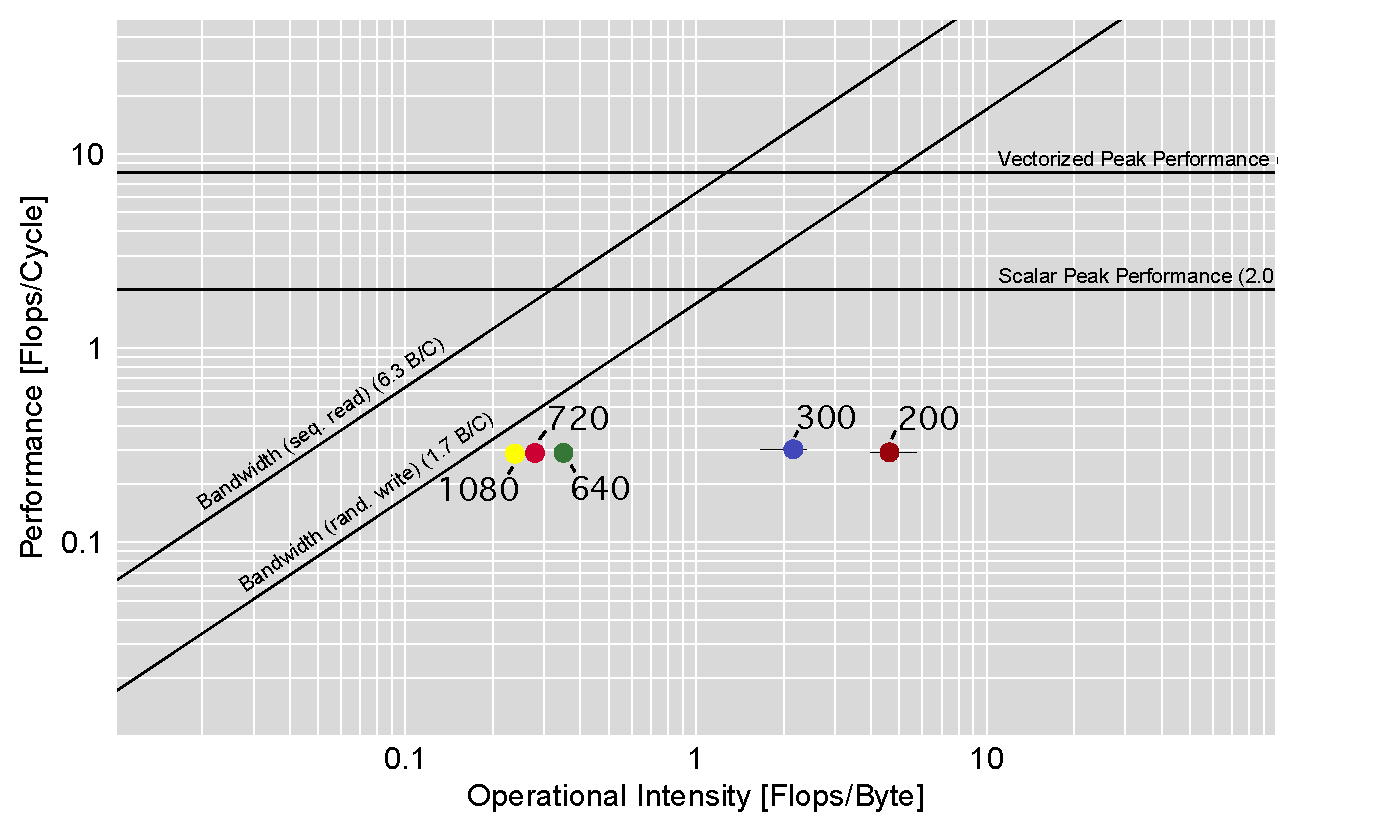
\includegraphics[width=0.85\textwidth]{figures/roofline}
    \caption{Roofline plot showing the performance of our vectorised code. }
    \label{fig:roofline}
\end{figure*}

\fixme{Write.}

\comment{
Here you evaluate your work using experiments. You start again with a
very short summary of the section. The typical structure follows.

\mypar{Experimental setup} Specify the platform (processor, frequency, cache sizes)
as well as the compiler, version, and flags used. I strongly recommend that you play with optimisation flags and consider also icc for additional potential speedup.

Then explain what input you used and what range of sizes. The idea is to give enough information so the experiments are reproducible by somebody else on his or her code.

\mypar{Results}
Next divide the experiments into classes, one paragraph for each. In the simplest case you have one plot that has the size on the x-axis and the performance on the y-axis. The plot will contain several lines, one for each relevant code version. Discuss the plot and extract the overall performance gain from baseline to best code. Also state the percentage of peak performance for the best code. Note that the peak may change depending on the situation. For example, if you only do additions it would be 12 Gflop/s
on one core with 3 Ghz and SSE and single precision floating point.

Do not put two performance lines into the same plot if the operations count changed significantly (that's apples and oranges). In that case first perform the optimisations that reduce op count and report the runtime gain in a plot. Then continue to optimise the best version and show performance plots.

{\bf You should}
\begin{itemize}
\item Follow the guide to benchmarking presented in class, in particular
\item very readable, attractive plots (do 1 column, not 2 column plots
for this class), proper readable font size. An example is below (of course you can have a different style),
\item every plot answers a question, which you pose and extract the
answer from the plot in its discussion
\end{itemize}
Every plot should be discussed (what does it show, which statements do
you extract).
}

\section{Conclusions}
\fixme{Write.}

In this report we presented a summary of optimization strategies for an edge preserving blurring filter. Even though the baseline implementation was already fast, we got an approximate $2x$ peformance gain in our final code version.

During the course of optimization we got rid of the primitive bottleneck which was the matrix transpose, by writing the data in transposed fashion directly. This allowed us to focus on the iterative part of the algorithm.

The way data is processed gives natural spatial locality and also instruction level paralellism, as 3 colour channels are stored contiguously but computed independently. This is also the reason why manual vectorization didn't give any performance improvement, as the pipeline of computation was already filled as much as the data allows.

We have attempted to analyze the performance bound of our code using roofline plots. However our fastest version is neither memory or compute bound, as we can see from the plot. This probably means that we are bound by some other factor. \comment{which we have no idea what it is :b}

\comment{
Here you need to briefly summarize what you did and why this is
important. {\em Do not take the abstract} and put it in the past
tense. Remember, now the reader has (hopefully) read the paper, so it
is a very different situation from the abstract. Try to highlight
important results and say the things you really want to get across
(e.g., the results show that we are within 2x of the optimal performance ... 
Even though we only considered the DFT, our optimization
techniques should be also applicable ....) You can also formulate next
steps if you want. Be brief.
}


\comment{
\section{Further comments}

Here we provide some further tips.

\mypar{Further general guidelines}

\begin{itemize}
\item For short papers, to save space, I use paragraph titles instead of
subsections, as shown in the introduction.

\item It is generally a good idea to break sections into such smaller
units for readability and since it helps you to (visually) structure the story.

\item The above section titles should be adapted to more precisely
reflect what you do.

\item Each section should be started with a very
short summary of what the reader can expect in this section. Nothing
more awkward as when the story starts and one does not know what the
direction is or the goal.

\item Make sure you define every acronym you use, no matter how
convinced you are the reader knows it.

\item Always spell-check before you submit (to me in this case).

\item Be picky. When writing a paper you should always strive for very
high quality. Many people may read it and the quality makes a big difference.
In this class, the quality is part of the grade.

\item Books helping you to write better: \cite{Higham:98} and \cite{Strunk:00}.

\item Conversion to pdf (latex users only): 

dvips -o conference.ps -t letter -Ppdf -G0 conference.dvi

and then

ps2pdf conference.ps
\end{itemize}

\mypar{Graphics} For plots that are not images {\em never} generate (even as intermediate step)
jpeg, gif, bmp, tif. Use eps, which means encapsulate postscript, os pdf. This way it is
scalable since it is a vector graphic description of your graph. E.g.,
from Matlab, you can export to eps or pdf.

Here is an example of how to get a plot into latex
(Fig.~\ref{fftperf}). Note that the text should not be any smaller than shown.

\begin{figure}\centering
% 	  \includegraphics[scale=0.33]{dft-performance.eps}
  \caption{Performance of four single precision implementations of the
  discrete Fourier transform. The operations count is roughly the
  same. {\em The labels in this plot are too small.}\label{fftperf}}
\end{figure}

}

% References should be produced using the bibtex program from suitable
% BiBTeX files (here: bibl_conf). The IEEEbib.bst bibliography
% style file from IEEE produces unsorted bibliography list.
% -------------------------------------------------------------------------
\bibliographystyle{IEEEbib}
\bibliography{bibl_conf}

\end{document}

